%----------------------------------------------------------------------------   
\chapter{Használt eszközök bemutatása}
%---------------------------------------------------------------------------- 

\section{Kubernetes}

A Kubernetes egy nyílt forráskódú konténer kezelő platform, amivel automatizálni
lehet a legtöbb feladatot, ami a fejlesztés, karbantartás vagy skálázással 
kapcsolatos. A Google fejlesztette eredetileg, de jelenleg a Cloud Native
Computing Foundation - CNCF vette át a karbantartását. 

Kubernetes fürtöt létrehozhatunk lokálisan a saját szerveren is vagy felhőben,
ami lehet publikus, privát vagy hibrid hozzáférésű. Viszont azt figyelembe 
kell venni, hogy egy Kubernetes fürtöt nem egyszerű kiépíteni lokálisan, 
szóval ha nem szükséges, akkor lehet használni felhőszolgáltatók Kubernetes 
motorjai, mint az Amazon AKS, Linode LKE vagy a Google GKE szolgáltatása.
Ilyenkor egy teljes fürtöt, ami az általunk beállított paramétereket használja.

\subsection{Felépítése}

Egy Kubernetes fürt kettő részből áll egy vezérlő- és egy adatsíkból, ahol a 
vezérlősíkban szereplő mester csomópontok tudják vezérleni az adatsíkban 
lévő dolgozó csomópontokat és a fejlesztők vagy üzemeltetők a mester által
hirdetett API-n keresztül képesek parancsokat kiadni. Míg a dolgozó 
csomópontokon futó alkalmazáshoz a felhasználók csak az általuk hirdetett 
Kube-Proxy segítségével tudnak hozzáférni. 

A kapcsolat mester és dolgozó között az API szerver és a Kubelet kommunikációján
alapul. Ha a fejlesztő szeretne egy új alkalmazást telepíteni a fürtön, akkor
szól az API szervernek, ami majd kiadja a megfelelő parancsokat a Kubelet-nek 
és majd az fogja a konténereket létrehozni. Amiről az API szervert értesítve 
tudja meg a fejlesztő, hogy amit csinált az létrejött. \\

A következőkben az alábbi ábra alapján részletesen kifejtem a Kubernetes 
részeit. 

\begin{figure}[!ht]
	\centering
	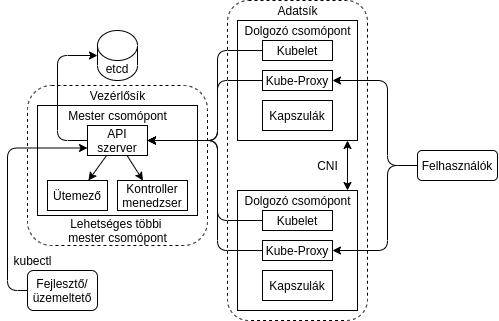
\includegraphics[width=1\textwidth, keepaspectratio]{figures/k8s_architecture.png}
	\caption{Kubernetes fürt felépítése}
	\label{fig:HVSpaces}
\end{figure}

\subsubsection{Vezérlősík}


\subsubsection{Adatsík}

\subsection{Fontos Kubernetes elemek}

Ahhoz, hogy jobban meglehessen érteni, mi hogyan működik a Kubernetes világban,
ezért az alábbi fogalmakat fontos ismerni:

\begin{itemize}
	\item \textbf{Vezérlősík (Controle Plane)}: Folyamatok gyűjteménye melyek 
	kontrollálják a Kubernetes csomópontokat.
	\item \textbf{Csomópont (Node)}: A vezérlősík által kiadott feladatokat 
	végrehajtó szerverek.
	\item \textbf{Kapszula (Pod)}: Több konténer gyűjteménye, melyek egyetlen
	csomóponton futnak és egy IP címem és más dolgokon osztoznak.
	\item \textbf{Replikációs vezérlő (Replication Controller)}: Kontrollálja,
	hogy egy kapszulából hány azonos fusson a fürtön.  Ezek a másolatok majdnem 
	mindenben azonosak egymással.
	\item \textbf{Szolgáltatás (Service)}: A hozzárendelt kapszulák, vagyis 
	végpontok között képes a forgalmat elosztani. Emellett címkék alapján 
	képes automatikusan új végpontokat regisztrálni vagy törölni.
	\item \textbf{Telepítő (Deployment)}: Deklaratívan frissíti a kapszulákat 
	és a replikációs vezérlőt. Így, ha valamilyen indok miatt egy kapszulában
	lévő konténer hibát generál, akkor újraindítja vagy esetlegesen törli a 
	kapszulát és egy teljesen újat indít. 
	\item \textbf{Egyéni erőforrás definíció (Custom Resource Definition)}:
	A Kubernetes API (Application Programming Interface) kiterjesztésére 
	lehet használni.
	\item \textbf{Operátor (Operator)}: Egy alkalmazás specifikus kontroller, 
	ami kibővíti a Kubernetes API funkcionalitását. 
	\item \textbf{Kubelet}: Csomópontokon futó szolgáltatás, ami a konténer 
	leírások alapján biztosítja, hogy a definiált konténerek fussanak.
	\item \textbf{kubectl}: Parancssoros eszköz, amivel a Kubernetes-t lehet 
	konfigurálni.
\end{itemize}

\section{L7mp}

Az L7mp egy több protokollt támogató szolgálatatás haló es porxy, amellyel 
könnyen lehet a legtöbb szállítás és alkalmazás réteg béli protokollt továbbítani
illetve fordítani. Esetünkben a szolgáltatás háló funkcionalitása lesz a 
fontosabb, de ettől függetlenül kitérek a proxy részére is, mert minden a 
legtöbb Kubernetes erőforrás használni fogja a proxy részét is. 

A szakdolgozat szempontjából még érdemes megemlíteni, hogy ez egy még nagyon 
erősen fejlesztés alatt álló projekt, szóval a vele megvalósított megoldások 
nem biztos, hogy tudják garantálni a megbízhatóságot. \\

Beszerzése ennek a szoftvernek rendkívül egyszerű. Ha csak a proxy-ra van 
szükség, akkor ugyan úgy telepíthető, mint bármelyik NPM (Node Package Manager)
csomag vagy használható Docker konténerként is, aminek a képfájlja elérhető 
ezzel a címkével: \textbf{l7mp/l7mp}. 

De a szolgáltatás háló használatához már muszáj Helm-t használni, amivel 
teljes Kubernetes architektúrákat lehet könnyedén megvalósítani. Ennek a 
menete megtalálható az L7mp oldalán is. 

\subsection{L7mp, mint proxy}

Működésében, nagyon hasonló az Envoy-hoz, ami egy a lyft által készített és 
nagyon sok helyen használt proxy. Azzal a különbséggel, hogy az L7mp inkább 
az alsóbb rétegbeli protokollokat támogatja, ezért a szállítási réteg legtöbb 
protokollja támogatva van és lehet bizonyos értékeik alapján irányítani a 
proxy-n áthaladó forgalmat. Példának okáért lehet olyat csinálni, hogy egy
Unix Domain Socket (UDS) foglalaton figyeli a forgalmat, majd azt WebSocket-re
átfordítva küldi tovább. 

Ezzel szemben nagyon sok olyan tulajdonsággal nem rendelkezik, ami megtalálható
az Envoy-ban. Ilyennek tudható be, hogy az alkalmazás réteg protokolljai nincsenek 
teljesen támogatva vagy nem rendelkeznek olyan szintű implementációval. Ami 
még egy nagyobb hátránya, hogy nem tud olyan gyors lenni az L7mp, mint az Envoy.
Ennek a legnagyobb oka, hogy az L7mp Node.js keretrendszerben íródott, ami a 
JavaScript miatt sokkal lassabb, mint a C++ nyelven íródott Envoy.

\subsubsection{Felépítése}

Mint már említve volt az L7mp rendkívül hasonlít az Envoy-ra és ez nincs másképp 
a felépítésben is. Szóval ennek a proxy-nak a használatához a következő 
építőköveket kell jobban ismerni: \textbf{Session}, \textbf{Listeners}, \textbf{Clusters}, \textbf{Endpoints}, \textbf{Rules}, \textbf{Routes}.\\

A Session (munkamenet) mindig akkor jön létre, amikor valamelyik Listener 
bejövő forgalmat kap. Erre azért van szükség, hogy a láncban meghatározott 
elemeknek mindig a megfelelő függvénye hívódjon meg és a hibák megfelelően 
legyenek kezelve. 

A Listener vagy magyarul figyelő úgy működik, mint egy szerver, ami bizonyos 
szempontok alapján figyelik a hozzájuk beérkező forgalmat és azt továbbítják
egy adott címre. Ezek a címek a Cluster-ek (fürtök) szoktak lenni, amiknek a 
működése közel azonos a Listener-ével, mivel ezek is a rajtuk beérkező forgalmat
adják tovább, azzal a kivétellel, hogy ezek nem láthatóak a proxy-n kívülről.

Végük a forgalom utolsó állomása az Endpoint vagyis végpont, ami már egy konkrét
cím, ahol figyel az általunk beállított alkalmazás. Fontos megjegyezni, hogy 
ezek az útvonalak kétirányúak, szóval a proxy képes kimenő forgalmat is ugyanúgy 
kezelni, mint a bejövőt. 

Amik a fentebb említett elemeket összeköti az a Rule (szabály) és a Route (irány),
A szabály által lehet különböző paraméterekre szűrni vagy hozzáadni. Ez azért egy 
nagyon hasznos funkció, mert ezáltal egy Session-n belül képes UDP forgalmat 
címkékkel ellátni és ezen címkék alapján megfelelő irányba továbbítani a 
forgalmat.

\subsubsection{Programozása}

Az L7mp indításához mindig biztosítani kell neki egy alapkonfigurációt, ami 
lehet általában egy L7mpController Listener-t és egy Cluster-t jelent, amin 
keresztül információkat tudunk szerezni az éppen futó proxy-ról vagy új 
elemeket lehet egyszerűen létrehozni. 

Új elemek hozzáadásához csak a proxy címére kell egy POST HTTP (HyperText Transfer 
Protocol) hívást indítani, aminek keretében a konfigurációt YAML (YAML Ain't Markup 
Language) vagy JSON (JavaScript Object Notation) formátumban tudjuk átadni.
Erre alább lehet látni egy nagyon egyszerű példát, ahol az L7mp a következő címen 
figyel: http://localhost:1234. 

\begin{lstlisting}
	curl -iX POST --header 'Content-Type:text/x-yaml' --data-binary @- <<EOF  http://localhost:1234/api/v1/listeners
	listener:
	  spec:
	    protocol: WebSocket
	    port: 2000
	  rules:
	    - action:
	        route:
	          destination:
	            spec:
  	              protocol: UDP
	              port: 3000
	            endpoints:
	              - spec:
	                  address: 127.0.0.1
	EOF
\end{lstlisting}

A fenti hívásban az látható, hogyan lehet egy Listener-t minden attribútumával 
létrehozni a proxy-n belül. Ez most a 127.0.0.1:2000-s címen figyel és minden 
bejövő forgalmat UDP-n továbbít a 127.0.0.1:3000-s címre. De ettől sokkal több
mindent is belehet állítani könnyedén. 

\subsection{L7mp, mint szolgáltatás háló}

Szolgáltatás háló alatt igazából egy olyan operátora kell gondolni, ami a Kubernetes
API-n (Application Programming Interface) keresztül képes L7mp proxy-k halmazát 
kezelni. Ezáltal könnyen tudjuk az L7mp-t, mint ingress gateway használni és 
mint sidecar az alkalmazás kapszulákban.

Ez az operátor három CRD-t használnak a L7mp proxy-k programozására, amik a következők:
\textbf{VirtualService}, \textbf{Target}, \textbf{Rule}. Ezek sorban a következő proxy 
elemeknek felelnek meg: \textbf{Listener}, \textbf{Cluster}, \textbf{Rule}. \\ 

Egy \textbf{VirtualService} az absztrakt megvalósítási egy szerver oldali foglalatnak címnek. 
Ezenfelül egy VirtualService mögött mindig áll egy Kubernetes szolgáltatás, ami 
szolgáltatja a végpontok címét vagy címkéit az elérhetőség miatt.

VirtualService részei: 

\begin{itemize}
	\item Egy szelektor, ami kiválasztja a definiált kapszulákat címkék alapján.
	\item Egy Listener, ami kezeli a beérkező forgalmat. 
	\item (Opcionális) Egy szabálylista, ami tartalmazhat újraírást, érték ellenőrzést
	és meghatározza a célt. 
	\item (Opcionális) További beállítások.  
\end{itemize}

A kliens oldali foglalatot mindig a \textbf{Target} valósítja meg, de beállíthatóak még a 
következő tulajdonságok is: terhelés elosztás, lokális cím lefoglalása, illetve 
meghatározhatnak még végpontot is, amihez a kliensnek csatlakoznia kellene. Ez 
lehet egy másik Target, konkrét cím vagy egy Listener is. Ezenfelül még meglehet 
határozni a bejövő és kimenő forgalom útját is. Így különböző útvonalakat lehet 
könnyen megvalósítani. 

Ha egy Target egyedi névvel rendelkezik, akkor más L7mp erőforrás könnyen 
felhasználhatja a névére való hivatkozással. Ez mind a három CRD-re igaz, de ha
nem határozunk meg egy konkrét nevet, akkor a rendszer automatikusan generál 
egyet minden erőforrásnak. 

%--------------
% PLACE OF RULE
%--------------